\documentclass[../draft.tex]{subfiles}

\begin{document}
    \chapter{Background}
    In this chapter, we introduce the necessary background.
    In \autoref{s:dataflow}, we explain the term static data flow analysis.
    We introduce concepts used to solve data flow problems precisely in \autoref{s:bigifds} and \autoref{s:ap}.
    We reason the need for a more manageable code representation in \autoref{s:jimple}.
    Finally, we introduce \textsc{FlowDroid}, the tool our work is based on, in \autoref{s:flowdroid}.

    \section{Static Data Flow Analysis}\label{s:dataflow}
    In the field of compilers, there is a distinction between static and dynamic.
    Static generally refers to something that is decided at compile-time, while dynamic refers to runtime decisions \cite{Aho1986}.
    The same distinction is also present for analyses.
    Dynamic analysis observes the program's runtime behavior, while static analysis works on a representation of the code.
    Both have different tradeoffs.
    Achieving good code coverage is a challenge in dynamic analysis.
    In contrast, a static analysis often can not infer runtime properties, hence follows paths never taken at runtime, also called \textit{infeasible paths} \cite{Arzt2017PhD}.
    Thus the dynamic analysis is an underapproximation and static analysis is an overapproximation.
    In the following, we only consider static analysis.

    Data flow analysis is a broad term for analyses that try to identify data flows through a program.
    Khedker \cite{Khedker2009} defines data flow analysis as follows:
    \begin{quote}
        \textit{Data flow analysis is a process of deriving information about the run time behavior of a program.}
    \end{quote}
    Data flow analyses are used in many different ways.
    Compilers use it to apply optimizations, others use it for software verification and it is also used for reverse-engineering \cite{Khedker2009}.
    A special kind of data flow analysis is taint analysis, which concepts might be familiar from code reviews.
    In taint analysis, the goal is to determine whether a particular variables' information contents flow through the program to another variable.
    Variables that contain valuable information are \textit{tainted}.
    This valuable information has to come from somewhere, the so-called \textit{sources}.
    Sources can be any expression but are often methods.
    Values produced from sources are considered tainted.
    On the other end, \textit{sinks} leak valuable information.
    A data flow between a source and a sink is called a \textit{leak} \cite{Arzt2017PhD}.
    For example, to detect apps tracking the user using taint analysis, sources could be methods returning a unique identifier and sinks could be methods that sent out data to the internet.
    When finding a leak, we know the receiving server can identify the device.

    There is also a categorization for data flow analyses.
    Sensitivities describe whether an analysis is capable of considering an aspect.
    There are five common sensitivities \cite{Khedker2009,Arzt2017PhD}:
    \begin{itemize}
        \item \textbf{Flow Sensitivity}: A flow-sensitive analysis can determine if a fact holds at a particular statement.
        \item \textbf{Context Sensitivity}: An interprocedural analysis can distinguish the context of a called method, e.g., knows the original call site at a return statement.
        \item \textbf{Object Sensitivity}: An analysis can distinguish field accesses on different objects.
        \item \textbf{Field Sensitivity}: An analysis can distinguish different field accesses on the same object.
        \item \textbf{Path Sensitivity}: An analysis takes conditional branches into account, e.g., the condition holds after the branch.
    \end{itemize}

    We also need a representation for the information the analysis gathered: the data flow fact.
    A \textit{data flow fact} is a logical assertion that is either true or false at a statement.
    Now, there are two different kinds of facts: may and must.
    For a must analysis, the fact must hold on all paths to this statement, while a may analysis only guarantees the fact holds on one path.
    The decision of which kind fits depends on the type of data flow analysis.
    Taint analyses like \textsc{FlowDroid} are based on the may analysis \cite{Arzt2017PhD}.

    The analysis direction of a data flow analysis is also decided by the problem to be solved.
    A live variables analysis computes whether a variable is read before written in the future to eliminate potential dead assignments.
    A backward pass traditionally solves the problem.
    On the other hand, a reaching definitions analysis finds out if a definition reaches a statement without an intermediate assignment, usually solved by a forward pass.
    Additionally, there are also data flow analyses for which the direction is a design choice.
    For example, program slicing identifies a slice, a subset of the program's statements, which influence a statement (backward pass) or are influenced by a statement (forward pass).
    Taint analysis, on the other hand, can be solved in both directions with the same results \cite{Khedker2009}.

    \section{IFDS}\label{s:bigifds}
    \subsection{Original Definition}\label{s:ifds}
    Interprocedural finite distributive subset (IFDS) problems are a special class of a data flow analysis problem.
    Generally, the solution to a data flow problem is the meet-over-all-paths (MOP) solution, which is undecidable \cite{Rice1953}.
    However, all problems adhering to IFDS can be transformed into a graph-reachability problem and consequently, the solution is computable in polynomial time.
    It is context-sensitive and flow-sensitive by default \cite{Reps1995}.

    % graph, Flow-Sensitive
    IFDS operates on a so-called exploded supergraph.
    Every node in the exploded supergraph is a tuple $\langle s, d \rangle$ of a statement $s$ in the interprocedural control-flow graph and a data flow fact $d$.
    The domain is typically the set of variables in the program.
    Edges between two nodes $\langle s, d \rangle$ and $\langle s', d' \rangle$ exist if $d$ propagated over $s$ yields $d'$ and $s'$ is a successor of $s$.
    Propagating facts along the control-flow graph already ensures flow-sensitivity.

    \begin{figure}[ht]
        \centering
        \begin{adjustbox}{max width=\columnwidth}
            \begin{lstlisting}[basicstyle=\itshape, mathescape, gobble=16, numbers=none,literate={->}{$\rightarrow$}{2}]
                matched -> ($_i$ matched )$_i$ matched | $\epsilon$
                valid -> valid ($_i$ matched | matched
            \end{lstlisting}
        \end{adjustbox}
        \caption{Context-Free Grammar proposed by Reps et al.\cite{Reps1995}}
        \label{lst:cfl}
    \end{figure}

    % Context-Sensitive
    To achieve context-sensitivity, Reps et al. proposed a context-free grammar (c.f. \autoref{lst:cfl}).
    Each call site gets a unique index, outgoing call edges are labeled with $(_i$ and incoming return edges are labeled with $)_i$.
    \textit{matched} ensures the correct return edge is taken and \textit{valid} models a partially balanced path, e.g., after a call for which the return is still pending.
    A path between two nodes is called \textit{valid} if the sequence of labeled edges is a string in \textit{valid} \cite{Reps1995}.
    Consider the example in \autoref{tikz:context}.
    After the first call to \code{bar}, the sequence is $(_1$, which is in \textit{valid}.
    Now, there are multiple return edges from \code{bar} but only $)_1$ is in \textit{matched}.
    Thus, only the $)_1$ edge is taken.
    MOP with this context-free language is also called meet-over-all-valid-paths (MOVP). MOVP increases the precision but does not compromise soundness ($\mathit{MOVP} \sqsubseteq \mathit{MOP}$).
    Still, the valid paths are an overapproximation because they also contain infeasible paths.

    \begin{figure}[ht]
        \centering
        \begin{tikzpicture}[auto,
            s/.style={},
            v/.style={draw, fill=black, circle, inner sep=0pt, minimum size=5pt},
            every node/.style={anchor=base west, align=left},
            every matrix/.style={column sep=2cm,row sep=0cm},
            vto/.style={->, >=stealth, thick}]
            \matrix[] {
                \node[s] (foo0) {\smallcode{void foo()\{}}; & \\
                \node[s] (foo1) {\smallcode{\ \ \ \ int i = 0;}}; & \\
                \node[s] (foo2) {\smallcode{\ \ \ \ int j = bar(i);}}; & \node[s] (bar0) {\smallcode{int bar(int p)\{}};\\
                & \node[s] (bar1) {\smallcode{\ \ \ \ return p + 42;}};\\
                \node[s] (foo3) {\smallcode{\ \ \ \ int k = bar(j);}}; & \node[s] (bar2) {\smallcode{\}}};\\
                \node[s] {}; &\\
                \node[s] {}; &\\
                \node[s] (foo4) {\smallcode{\ \ \ \ return k;}}; &\\
                \node[s] (foo5) {\smallcode{\}}}; &\\
            };

            \draw[vto, color=darkgreen] (foo2) to[out=0, in=135] node [midway, above, sloped]{$(_1$} (bar0);
            \draw[vto, color=darkgreen] (bar1) to[out=-100, in=45] node [midway, above, sloped]{$)_1$} (foo3);
            \draw[vto, color=orange] (foo3) to[out=0, in=150] node [midway, above, sloped]{$(_2$} (bar0);
            \draw[vto, color=orange] (bar1) to[out=-90, in=45] node [midway, above, sloped]{$)_2$} (foo4);
        \end{tikzpicture}
        \caption{Context-Sensitivity using a Context-Free Language}
        \label{tikz:context}
    \end{figure}

    % flow functions
    To propagate facts over statements, we need to define rules on how the data flow changes when observing a statement.
    These rules are called flow functions.
    There are four types of flow functions: \cite{Reps1995}
    \begin{itemize}
        \item \textbf{Call Flow}: Edges from call statement into a method. The flow function maps the facts visible in the callee into it.
        \item \textbf{Return Flow}: Edges returning from a method. The flow function maps the facts visible in the caller out of the callee.
        \item \textbf{Call To Return Flow}: Edges over a call statement. The flow function maps the facts not visible in the callee over the call statement.
        \item \textbf{Normal Flow}: The default case. Handles edges over every other statement, for example, assignments.
    \end{itemize}
    The incoming set of facts is all predecessors' outgoing facts merged using a merge operator $\sqcap$:
    $$
        in(s) := \bigsqcap_{p \in Preds(s)} out(p)
    $$
    % introduce taints
    Now, we also want to introduce new facts.
    For that reason, the domain contains a zero fact and all nodes with $d=\textbf{0}$ are always reachable; thus, the zero fact is a tautology.
    Whenever we want to introduce a fact, we can model this in the flow function by deriving such facts from the zero fact  \cite{Reps1995}.
    For example, in taint analysis, the flow functions map zero facts at sources to a tainted variable.

    % summaries
    IFDS also utilizes summaries.
    After returning from a method, the algorithm solved a subproblem for which it remembers the results to be applied later.
    So, the proposed tabulation algorithm for solving the realizable path problem is a dynamic algorithm \cite{Reps1995}.

    % Fix point
    Eventually, the worklist is empty as there are no facts to propagate anymore and the analysis will terminate.
    There are two ways for a fact to be not propagated further.
    Either a flow function killed the fact or the same fact was already observed at a statement, meaning the IFDS analysis reached a fixpoint \cite{Reps1995}.

    However, we already started this section, hinting not all problems can be formulated in the IFDS framework.
    The restrictions the problems have to abide by are eponymous in IFDS and explained in the following paragraphs.

    \paragraph{Distributive} The flow function must be distributive over the merge operator.
    Formally, $f(x \sqcap y) = f(x) \sqcap f(y)$ must hold at any time.
    Informally speaking, it does not matter whether facts get merged before or after applying the flow functions.
    Distributiveness is essential for the correctness of IFDS because only if the flow functions are distributive, the maximum fixed point (MFP) equals MOP and MFP is computable in polynomial time \cite{Khedker2009,Reps1995}.

    \paragraph{Finite} Another restriction is that the set of data flow facts has to be finite.
    Let us go by a counterexample of what IFDS is not capable of: Answering "Which value is stored in variable x at statement s?".
    Now the data flow fact is a tuple of the variable together with the stored value $\langle x, v \rangle$.
    Consider \autoref{lst:ifdsfinite}.
    $x$ is initialized to an empty string and in every loop iteration, \code{\"a\"} gets appended to the string.
    The value of x changes every time and never repeats itself.
    In theory, the algorithm will never observe a taint twice in line 4.
    Because the algorithm can not reach a fixpoint, it will not terminate.
    In practice, every data type is bounded either by the heap or stack size, but the domain is cubic in the time-complexity $O(|E| \cdot |D|^3)$ making IFDS infeasible for large domains \cite{Reps1995}.

    \begin{figure}[ht]
        \centering
        \begin{subfigure}[b]{0.45\textwidth}
            \centering
            \begin{adjustbox}{max width=\columnwidth}
                \begin{lstlisting}[gobble=20]
                    void main() {
                        String x = "";
                        while (condition)
                            x += "a";
                    }
                \end{lstlisting}
            \end{adjustbox}
            \caption{Code}
        \end{subfigure}
        \qquad
        \begin{subfigure}[b]{0.45\textwidth}
            \centering
            $$
                \begin{aligned}
                    \langle x, \epsilon \rangle &\rightarrow \langle x, a \rangle\\
                    \langle x, a \rangle &\rightarrow \langle x, aa \rangle\\
                    \langle x, aa \rangle &\rightarrow \langle x, aaa \rangle\\
                    &\dots
                \end{aligned}
            $$
            \caption{Taint Derivations}
            \label{lst:ifdsfinite_b}
        \end{subfigure}
        \caption{Finiteness example}
        \label{lst:ifdsfinite}
    \end{figure}

    \paragraph{Subset} Data flow frameworks need to deal with merging the outcoming sets to a single incoming set.
    Essentially, to formalize the approximation and satisfy ordering constraints, data flow frameworks rely on lattices \cite{Khedker2009}.
    IFDS also defines an underlying lattice on the powerset of the domain.
    The lattice ordering must be set inclusion.
    Therefore, the merge operator is set union or set intersect.
    Now recall may and must from \hyperref[s:dataflow]{the last subsection}.
    Here we can see the connection between the merge operator and may or must.\\
    The paper by Reps et al. later decides on set union due to the duality of must and may not \cite{Reps1995}.
    This decision is also efficient in practice, as discussed in the \hyperref[s:ifdspractical]{following subsection}.


    \subsection{Practical Extensions}\label{s:ifdspractical}
    The original definition is inefficient in practice.
    Among others, Naeem et al. proposed practical extensions to the IFDS framework to perform better in practice \cite{Naeem2010}.

    The original algorithm demands a fully built exploded supergraph.
    Even in moderate programs, the domain can get quite large.
    As the nodes in the exploded supergraph are the cross-product of the domain and interprocedural call-graph nodes, it is infeasible to generate the full graph beforehand.
    Because there is no way to know before which part of the supergraph the analysis demands, they propose to generate it ad-hoc.
    That also removes the restriction on a small domain.
    Now IFDS is also feasible if the domain's encountered subset is small enough \cite{Naeem2010}.
    The restrictions on the domain set can be loosened even more.
    Bodden suggests the domain can be infinite in practice.
    Only the observed facts must adhere to the ascending-chain condition over the flow functions when using the on-demand supergraph \cite{Bodden2012}.

    Also, the original IFDS definition ignores the type structure of the programming language.
    Type information can be used to kill facts due to impossible casts.
    Also, facts with the same variable but different types can be merged with the superclass as its new type \cite{Naeem2010}.

    Furthermore, the original definition starts the IFDS algorithm at the entry point of the interprocedural call-graph.
    As described in \autoref{s:ifds}, a flow function can derive an initial fact from the zero fact if needed.
    If the methods where initial facts will be introduced are known a priori, the supergraph can be traversed without applying flow functions until such a method is found on the path.
    This optimization introduces unbalanced problems where a method returns but no corresponding call site is found, which can be solved by a small extension to the tabulation algorithm.
    Lerch et al. first described the extension \cite{Lerch2015} and it is also present in \textsc{FlowDroid} \cite{Arzt2017PhD}.

    Another optimization is possible if the merge operator is set union thanks to the $A \subseteq A \cup B$ property of set union.
    There is no need to wait for other predecessors to finish as a set is always a subset of a union with itself and another set.
    Hence, the IFDS solver can skip the $in$-set construction and immediately propagate the outcoming facts as singleton sets, sometimes referred to as point-wise propagation.
    Especially parallelized IFDS implementations benefit from point-wise propagation \cite{Rodriguez2011}.

    \section{Access Paths}\label{s:ap}
    We have already seen IFDS fulfills context- and flow-sensitivity by default.
    Now, a precise analysis for Java also needs object- and field-sensitivity.
    Thus, we also need to model the heap.

    Access paths are one possible heap model.
    They consist of a list of field dereferences linked to a tainted variable of a reference type \cite{Khedker2009}.
    Note, this increases the domain size because now not only "object $o$ is tainted" is a data flow fact, but also all of its fields can be tainted.
    Especially when encountering recursive data structures with loops such as doubly-linked lists, this gets problematical.
    Consider \autoref{lst:infiniteap}, the loop would let the observed domain grow indefinitely and never reach a fixpoint.
    As a solution, access paths are limited in length, which is also called $k$-limiting, whereas the constant $k$ is the maximum access path length.
    If an access path passes this length, it is cut off and the entire last reference is considered tainted.
    This cut-off comes with a loss of precision \cite{Jones1979}.
    Consider again \autoref{lst:infiniteap}.
    With $k=2$ the analysis would reach the fixpoint $lst.next.prev.*$ after two iterations.

    \begin{figure}[ht]
        \centering
        \begin{subfigure}[b]{0.45\textwidth}
            \centering
            \begin{adjustbox}{max width=\columnwidth}
                \begin{lstlisting}[gobble=20]
                    while (condition) {
                        lst = lst.next.prev;
                    }
                \end{lstlisting}
            \end{adjustbox}
            \caption{Code}
        \end{subfigure}
        \qquad
        \begin{subfigure}[b]{0.45\textwidth}
            \centering
            \small
            $$
            \begin{aligned}
                &lst& &\rightarrow lst.next.prev\\
                &lst.next.prev& &\rightarrow lst.next.prev.next.prev\\
                & & &...
            \end{aligned}
            $$
            \normalsize
            \caption{Access Path Iterations}
        \end{subfigure}
        \caption{Infinite Access Path}
        \label{lst:infiniteap}
    \end{figure}

    Although with $k$-limiting, the algorithm terminates, it does have another problem.
    After a loop like in \autoref{lst:infiniteap}, the access path is polluted with a dereference chain to its base object even though the $next.prev$ dereference could be omitted without precision loss.
    As a solution, Deutsch proposed symbolic access paths, which try to eliminate loops in access paths \cite{Deutsch1994}.
    In practice, Deutsch's approach needs some adaptions as he only considered fields but not base objects and he defines loops simply by type \cite{Arzt2017PhD}.
    With symbolic access paths $k$-limiting is theoretically obsolete but still often applied to speed up the analysis.

    \section{Intermediate Representations}\label{s:jimple}
    Most compilers these days use intermediate representations (IRs).
    IRs are an equivalent representation of the source code but are less complex and more regular and are typically not architecture-dependent.
    They are often in an interchangeable format and can be saved as text to be used by various tools \cite{Thain2019}.
    Such an IR allows compilers to apply machine-independent optimizations to the code without worrying about complex expressions in the source code or reimplementing the optimization for each architecture.

    The Java Virtual Machine (JVM) also operates on an IR called Java bytecode.
    The JVM is mostly stack-based and so is the Java bytecode.
    In \autoref{lst:jvmstack} is an example of a simple code snippet translated to Java bytecode.
    Simple expressions such as \code{c = a + b} translate into multiple statements and there is no fixed length of an expression in the bytecode.
    The analysis would also have to reconstruct the expressions ad-hoc.
    Furthermore, Java bytecode has over 200 possible instructions\footnotemark{}, which need to be considered and only knows primitive types and references.
    Concluding, stack-based IRs are suitable for just-in-time interpretation but inconvenient for data flow analysis \cite{Valleerai2004}.
    \footnotetext{Source: \url{https://docs.oracle.com/javase/specs/jvms/se8/html/} (visited on 17.04.2021)}

    \begin{figure}[ht]
        \centering
        \begin{subfigure}[b]{0.45\textwidth}
            \centering
            \begin{lstlisting}[gobble=16]
                int a = 21;
                int b = 21;
                int c = a + b;
            \end{lstlisting}
            \caption{Java code}
            \label{lst:jvmstack_a}
        \end{subfigure}
        \hfill
        \begin{subfigure}[b]{0.45\textwidth}
            \centering
            \begin{lstlisting}[gobble=16]
                bipush 21 // push 21
                istore_1  // store in register 1
                bipush 21 // push 21
                istore_2 // store in register 2
                iload_1 // push a
                iload_2 // push b
                iadd // pop a & b and push a + b
                istore_3 // store in register 3
            \end{lstlisting}
            \caption{Java bytecode}
            \label{lst:jvmstack_b}
        \end{subfigure}
        \caption{Java bytecode example}
        \label{lst:jvmstack}
    \end{figure}

    A more convenient representation for static analysis is three-address codes.
    Each statement consists of up to three operands and is either an assignment or a control-flow statement.
    Operands are represented by variables instead of registers or stacks.
    Such a representation fixes the expression length to be better suited for static analysis than assembly. It also reduces the possible combinations to a manageable amount compared to the source code written by a human \cite{Aho1986}.

    Jimple is a three-address intermediate representation and can be constructed from the Java and Dalvik bytecode, the IR used for Android apps.
    It is a high-level representation and its syntax is close to Java.
    Complex statements are split up into multiple statements.
    For example, there can be only one field reference per statement and arguments are always local variables or constants \cite{Valleerai2004}.
    This groundwork dramatically reduces the possible cases the data flow analysis needs to consider and eases the analysis.

    \section{FlowDroid}\label{s:flowdroid}
    \textsc{FlowDroid} is a precise context-, flow-, object- and field-sensitive static taint analysis tool for Android apps\cite{Arzt2014}.
    Since its initial release in 2014, it is actively maintained and gained traction in research and academia\footnotemark{}.
    It is based on Soot, a Java optimization framework, which later has been extended for static analysis \cite{Lam2011}.
    Soot provides the call graph and the conversion from Java and Dalvik bytecode to Jimple, the intermediate representation of choice for \textsc{FlowDroid} \cite{Arzt2017PhD}.
    \footnotetext{Source: \url{https://github.com/secure-software-engineering/FlowDroid} (visited on 17.04.2021)}

    Androids activity-lifecycle concept does not have a single entry point; instead, multiple callbacks are a possible entry point.
    Also, an Android app can contain multiple components and register callbacks in various of Android's standard libraries.
    \textsc{FlowDroid} models the entire Android lifecycle to be precise and generates a dummy main method to provide a single entry point for the call graph generation.
    \cite{Arzt2014}.

    \begin{figure}[tbp]
        \centering
        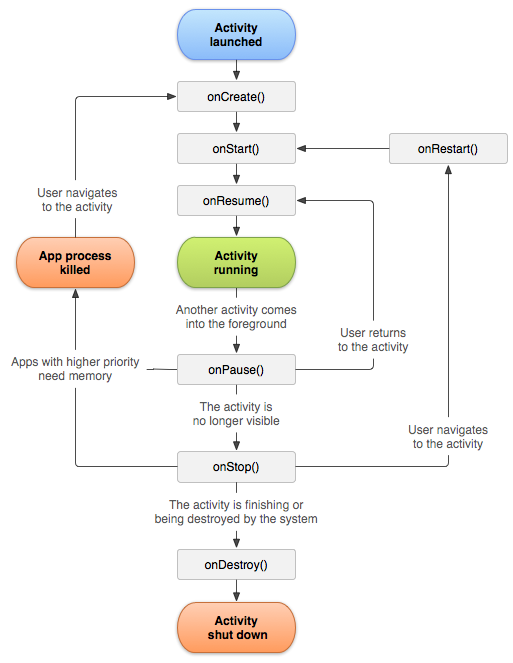
\includegraphics[width=0.35\textwidth]{figs/activity_lifecycle.png}
        \caption{Activity Lifecycle\protect\footnotemark}
        \label{f:activity}
    \end{figure}
    \footnotetext{Source: \url{https://developer.android.com/guide/components/activities/activity-lifecycle} (visited on 17.04.2021)}

    \textsc{FlowDroid} inherits flow- and context-sensitivity from IFDS and the object- and field-sensitivity from symbolic access paths. To provide precise results even with aliases in use, \textsc{FlowDroid} comprises an alais analysis. The alias analysis is encoded as another IFDS problem and resolves all encountered aliases on-demand. The two IFDS analyses are intertwined to maintain flow- and context-sensitivity between both analyses\cite{Arzt2014}.

    The implementation of \textsc{FlowDroid} is modular, easily extensible and offers many additional features.
    Two of them are noteworthy for this work: native call handler and taint wrappers.
    As both Java and Android allow calling native methods, \textsc{FlowDroid} also needs to model those cases.
    It currently does not support the analysis of those methods but contains rules for essential methods.
    The second feature is taint wrappers.
    They allow defining rules for methods, e.g., from a commonly used feature such as StringBuilder, which allows the taint analysis to skip the method and apply a summary \cite{Arzt2014}.
    StubDroid, an extension to FlowDroid by Arzt et al., allows precomputing summaries using \textsc{FlowDroid} and serializes them in an XML format for tool-independent use.
    These summaries are handy for real-world applications where third-party libraries are often used \cite{Arzt2016}.
\end{document}